\scanpage{121}

\figure{
\begin{tikzpicture}
\node[anchor=west] at (0,0) {corps de \# :};
\draw[dashed] (0,-.25)--(2.1,-.25);
\end{tikzpicture}}

\[
\operatorname{Gal}(\bar K/K)^{ab}
\longleftrightarrow
\pi_0(\mathbb A^*/K^*)=\text{limite projective des}
\]
$U\backslash\mathbb A^*/K^*$ pour $U$ sous-groupe ouvert d'indice fini de
\[
\prod_{v\mid\infty}K_v^*\times
\prod_{v\nmid\infty}O_v^*
\]

(pour
\[
U=
\prod_{v\text{ réel}}\mathbb R^{+*}
\times\prod_{v\text{ complexe}}\mathbb C^*
\times\prod_{v\nmid\infty,\ v\notin S}O_v^*
\times\prod_{v\in S}(1+m_v^{f_v})^*,
\]
ce quotient est le groupe des $\prod m_v^{f_v}$-classes d'idéaux stricts : le groupe des idéaux premiers à $S$, avec l'équivalence $a\sim b$ si $a=\alpha b$ avec $\alpha\in K^*$, $S$-entier, positif aux places réelles, $\alpha\equiv1\ (m_v^{f_v})\quad\forall v\in S$)

Il est souvent utile de savoir que, d'après Chevalley, tout sous-groupe d'indice fini du groupe des $S$-unités $H^0(\operatorname{Spec}O-S,O^*)$ \deleted{contient} contient un sous-groupe défini par une condition de congruence : $x\equiv1\ (b)$, $b$ idéal $\ne0$ convenable.

\uline{Local-global}

\diagram{\begin{tikzcd}[ampersand replacement=\&,column sep=huge,row sep=large]
\operatorname{Gal}(\bar K_v/K_v)^{ab}
\arrow[d,"{\substack{\text{groupe de}\\\text{décomposition}}}"']
\&K_v^*\arrow[l]\arrow[d]\\
\operatorname{Gal}(\bar K/K)^{ab}
\&\mathbb A^*/K^*\arrow[l]
\end{tikzcd}}

\begin{center}
\figure{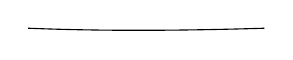
\begin{tikzpicture}[x=1cm,y=1cm]\draw (0,0) .. controls (1,-.04) and (2,-.03) .. (3,0);\end{tikzpicture}}
\end{center}

Pour la multiplication complexe, le théorème fondamental est celui de Shimura et Taniyama. Voici la façon de l'énoncer que je préfère (sauf qu'on ne parle pas assez de motifs).

Soit : $K$ un corps extension quadratique totalement imaginaire d'un corps de nombres totalement réel $F$.
\[
\unsure{g|q}=[F:\mathbb Q]
\]

\margin{121}
